\documentclass{article} % say
\usepackage{tikz}
\begin{document}
We are working on
\begin{tikzpicture}
\draw (-1.5,0) -- (1.5,0);
\draw (0,-1.5) -- (0,1.5);
\end{tikzpicture}.

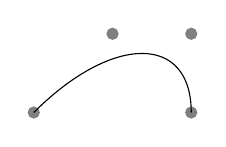
\begin{tikzpicture}
\filldraw [gray] (0,0) circle [radius=2pt]
(1,1) circle [radius=2pt]
(2,1) circle [radius=2pt]
(2,0) circle [radius=2pt];
\draw (0,0) .. controls (1,1) and (2,1) .. (2,0);
\end{tikzpicture}

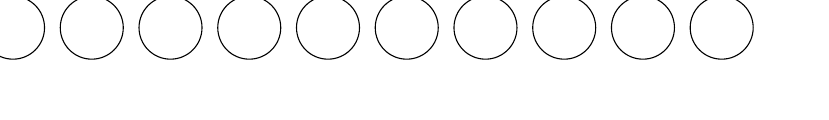
\begin{tikzpicture}
\tikz \foreach \x in {1,...,10}
\draw (\x,0) circle (0.4cm);
\end{tikzpicture}

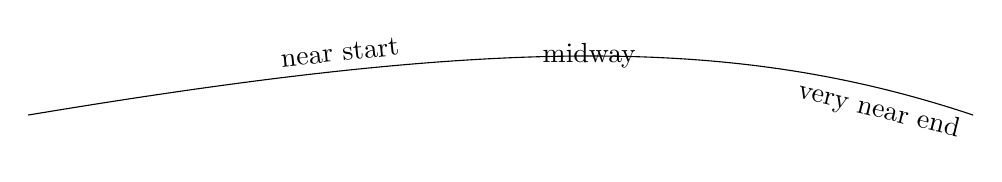
\begin{tikzpicture}
\draw (0,0) .. controls (6,1) and (9,1) ..
node[near start,sloped,above] {near start}
node {midway}
node[very near end,sloped,below] {very near end} (12,0);
\end{tikzpicture}

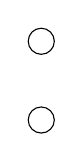
\begin{tikzpicture}
  \path (0,2) node [shape=circle,draw] {}
        (0,1) node [shape=circle,draw] {};
\end{tikzpicture}

\begin{tikzpicture}
  \draw (0,0) .. controls (-1,0.5) and (-3,3) .. (-3,6)
  node foreach \p in {0,0.1,...,1} [pos=\p,circle,radius=5pt,fill=white,draw] {};
  \draw (-3,6) circle [radius=10pt,fill=red] .. controls (-3,9) .. (-2,12)
  node foreach \p in {0.1,0.2,...,1} [pos=\p,circle,radius=5pt,fill=white,draw] {};
\end{tikzpicture}


\begin{tikzpicture}
 \draw (0,0) -- (1,0) -- (0.5,-1) -- cycle;
 \draw (0,0) .. controls (-11,13) and (12,13) .. (1,0)
 node foreach \p in {0.2,0.4,...,0.8} [pos=\p,circle,radius=10pt,fill=white,draw] {};
\end{tikzpicture}


\begin{tikzpicture}
[bigBead/.style={circle,draw=blue!50,fill=white,thick,
inner sep=0pt,minimum size=6mm}]
  \draw (0,0) -- (1,0) -- (0.5,-1) -- cycle;
  \node[bigBead] (firstOFbead)  at (-4,6) {};
  \node[bigBead] (secondOFbead) at (-2.5,12) {};
  \node[bigBead] (thirdOFbead)  at (3.5,12) {};
  \node[bigBead] (fourthOFbead) at (5,6) {}; 
  \draw (0,0) .. controls (-1,0) and (-4,5) .. (firstOFbead)
    foreach \t in {0.09,0.18,...,0.9} {
       pic [draw=blue!50,fill=white,pos=\t] {code={\path [pic actions] circle [radius=5pt];}}};
  \draw (firstOFbead) .. controls (-4,7) and (-3.5,11) .. (secondOFbead)
    foreach \t in {0.09,0.18,...,0.9} {
       pic [draw=blue!50,fill=white,pos=\t] {code={\path [pic actions] circle [radius=5pt];}}};
  \draw (secondOFbead) .. controls (-1.5,13) and (2.5,13) .. (thirdOFbead)
    foreach \t in {0.09,0.18,...,0.9} {
       pic [draw=blue!50,fill=white,pos=\t] {code={\path [pic actions] circle [radius=5pt];}}};
  \draw (thirdOFbead) .. controls (4.5,11) and (5,7) .. (fourthOFbead)
    foreach \t in {0.09,0.18,...,0.9} {
       pic [draw=blue!50,fill=white,pos=\t] {code={\path [pic actions] circle [radius=5pt];}}};
  \draw (fourthOFbead) .. controls (5,5) and (2,0) .. (1,0)
    foreach \t in {0.09,0.18,...,0.9} {
       pic [draw=blue!50,fill=white,pos=\t] {code={\path [pic actions] circle [radius=5pt];}}};
\end{tikzpicture}

\end{document}

